% Placeholder content for Chapter 3.
% \lipsum[3]

% \documentclass[final,5p,times,number]{elsarticle}
% \usepackage[T1]{fontenc}
% \usepackage[labelfont=bf,justification=raggedright,singlelinecheck=false]{caption}
% \usepackage{natbib}
% \usepackage{graphicx}
% \usepackage{amsmath, amssymb, amsthm}
% \usepackage{tabularx}
% \usepackage{caption}
% \usepackage{enumitem}
% \usepackage{array}
% \usepackage{float}
% \usepackage{multicol}
% \usepackage{multirow}
% \usepackage{xcolor}
% \usepackage[flushleft]{threeparttable}
% \usepackage{booktabs}

% \usepackage{adjustbox}
% \usepackage[hyphens]{url}
% \usepackage[breaklinks,hidelinks]{hyperref}
% \usepackage{siunitx}
% \usepackage{balance}
% \usepackage{xcolor}
% \usepackage[]{threeparttable}

% \usepackage{lineno}
% \linenumbers


% \newcommand{\etal}{\textit{et al}. }
% \newcommand{\etal}{et al. }
% \newcommand{\ie}{i.e., }
% \newcommand{\eg}{{e.g., }}

% \setlength{\emergencystretch}{2em}

% \journal{Automation in Construction}

% \begin{document}
% % \begin{linenumbers}
% \begin{frontmatter}



%\title{Road Damage Detection Using Detection Transformers}

%\title{Road Damage Detection: Evaluating State-of-the-Art Object Detection Models}
%\title{A Benchmark Study of Deep Learning Models for Road Damage Detection}
% \title{Road Damage Detection using Deep Learning}
\title{Deep Learning Models for Automated Road Damage Detection: A Comprehensive Evaluation, Insights and Future Directions}
%\title{Road Damage Detection using Deep Learning: Benchmarking, Challenges, and Future Scope}

% \author[inst1]{Suhail Najeeb}
% \author[inst1]{Aravinda S. Rao}
% \author[inst1]{Nandakishor Desai}
% \author[inst2]{Nhat Vo}
% \author[inst2]{Subhash Challa}
% \author[inst1]{Marimuthu Palaniswami}


% \affiliation[inst1]{organization={Department Electrical and Electronic Engineering},%Department and Organization
%             addressline={The University of Melbourne}, 
%             city={Melbourne},
%             postcode={3010}, 
%             state={Victoria},
%             country={Australia}
%             }

% \affiliation[inst2]{organization={SenSen Networks Ltd},%Department and Organization
%            addressline={Unit 2, 570 City Road}, 
%            city={South Melbourne},
%            postcode={3205}, 
%            state={Victoria},
%           country={Australia}}

% \begin{abstract}

Road damage detection plays a crucial role in ensuring effective maintenance of infrastructure and ensuring public safety. In recent years, computer vision techniques, especially deep learning approaches, have shown promising directions in addressing this problem. In this study, we present a comprehensive evaluation of six state-of-the-art deep learning models for road damage detection. We utilize an open-source dataset designed explicitly for this task and compare the performance of models including Faster Region-Based Convolution Neural Network (Faster R-CNN), Single Shot Detector (SSD), You Only Look Once (YOLO) version 8 (YOLOv8), YOLOv11, Detection Transformer (DETR), Deformable-DETR, and RT-DETR. In this article, we present a comprehensive review of state-of-the-art deep learning models for detecting road damage. We provide in-depth analysis using various performance metrics and comparisons. We also offer vital findings, limitations, and future directions. Our findings represent a significant step toward streamlining and improving automated road damage detection mechanisms.

% \end{abstract}

% %%Graphical abstract
% \begin{graphicalabstract}
% 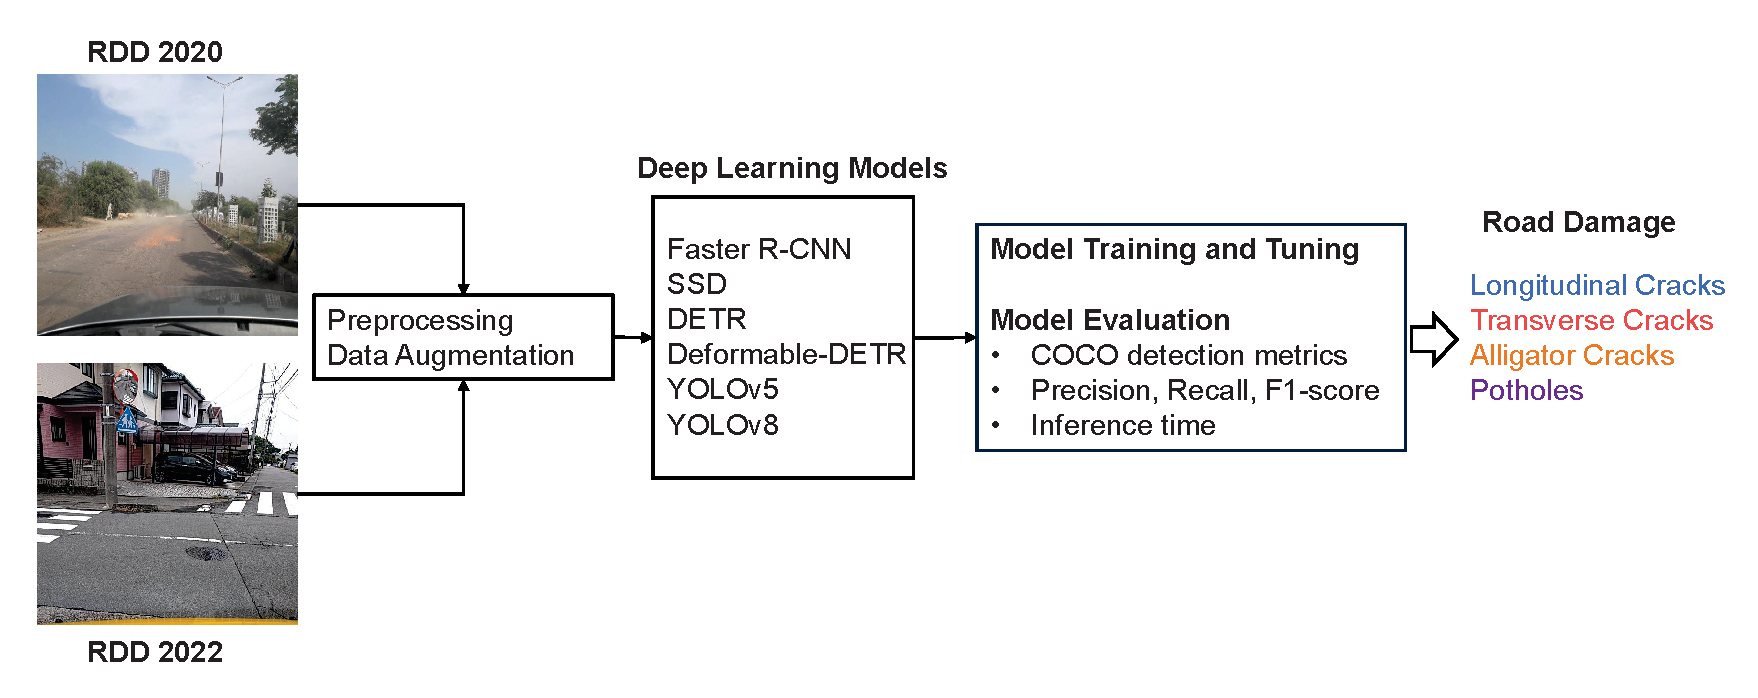
\includegraphics[width=0.95\textwidth]{figs/Figure_overview.eps}
% \end{graphicalabstract}

%%Research highlights
% \begin{highlights}
% \item Comprehensive evaluation of six state-of-the-art object detection models
% \item In-depth comparison of models using two public datasets in detecting road damages
% \item Outline challenges and limitations of datasets, models, and real-world deployments
% \item Future research roadmap for automated road damage detection through critical insights 
% \end{highlights}

% \begin{keyword}
% %% keywords here, in the form: keyword \sep keyword
% Pavement damages \sep automated road maintenance \sep deep learning \sep computer vision \sep road damage detection
% %% PACS codes here, in the form: \PACS code \sep code
% %\PACS 0000 \sep 1111
% %% MSC codes here, in the form: \MSC code \sep code
% %% or \MSC[2008] code \sep code (2000 is the default)
% %\MSC 0000 \sep 1111
% \end{keyword}

% \end{frontmatter}

%% \linenumbers

%% main text
\sloppy
\section{Introduction}

Road transport infrastructure is essential for any modern society and serves as the backbone of economic growth and development \cite{rojo2018impact}. It provides access to critical services and is a crucial component for moving goods, services, and markets. However, factors such as budgetary constraints, underinvestment in upgrades, and delayed maintenance can lead to the degradation of road infrastructure \cite{gopalakrishnan2018deep}. Furthermore, the recent increase in the number of vehicles has also resulted in pavement distress \cite{chen2016development}. Damaged roads cause ecological, economic, and social damage, such as the high costs of vehicle repairs, traffic congestion, accidents, time delays, and additional fuel consumption and emissions \cite{han2020intelligent}. 

Due to the nature of road infrastructure, it is exposed to various types of damage and deterioration, which can be caused by different factors such as traffic load, structural materials, environment, weather, aging, and construction activities \cite{bhandari2023understanding, arya2021deep}. These factors affect the condition and longevity of the pavement. Among these factors, traffic load has a significant influence on pavement performance and causes difficulties in maintaining pavement service life. Therefore, it is essential to maintain the road infrastructure in good condition to ensure the safety of road users and minimize the cost of maintenance.

Pavement damage is an essential aspect of maintaining road infrastructure. There are different ways to evaluate pavement conditions. The evaluation process can be manual, semi-automated, or fully automated \cite{arya2021deep}. Manual pavement condition evaluation is performed by visually inspecting the road surface by trained personnel, which is time-consuming and costly. The manual approach also raises some safety concerns, requiring the person to be on the road surface. Semi-automated evaluation involves taking images of the road surface from a vehicle-mounted camera and evaluating it at a later time to determine the condition of the pavement \cite{zalama2014road, pierce2013practical}. This approach is safer and more efficient compared to the manual process, as it does not require the person to be on the road surface. However, the processing of the images is still done manually, which is time-consuming. Fully automated pavement condition evaluation involves sophisticated sensors such as laser scanners, road profilers, Light Detection and Ranging (LiDAR), and high-resolution cameras that can be used to capture intricate details of the road surface to determine the condition of the surface \cite{eisenbach2017get, guan2021automated}. However, these sensors are costly and difficult to deploy on a large scale.

Recent developments in mobile devices have made it inexpensive to capture images of the road surface using a vehicle-mounted mobile device and process the images using computer vision techniques to determine the condition of the pavement \cite{mertz_city, varadharajan_vision}. This provides a cost-effective and efficient approach to assessing the state of the pavement distress. Arya \etal \cite{arya_grddc20, arya2021deep} have explored the efficacy of combining training data from different sources to achieve better results in the detection problem of road damage. More recently, the Road Damage Detection (RDD) 2022 dataset \cite{arya_rdd2022} was introduced, which is a richer dataset that contains images of road surfaces from different countries around the world. This dataset allows further research to explore the efficacy of training deep learning models using data from other sources.

Several research challenges need to be addressed to achieve a robust and reliable solution to the problem of road damage detection. Due to the nature of the different damages and cracks on the road surface, the target objects to be detected are unique and specific to the problem of detecting road damage. Therefore, selecting an appropriate and efficient deep learning model is crucial to achieving good results. In this article, we present a comprehensive review of state-of-the-art deep learning models for detecting road damage. We provide an in-depth analysis using various performance metrics and comparisons. We also provide key findings, limitations, and future directions. Our key contributions include:
\begin{enumerate}[noitemsep,topsep=0pt]
    \item \textbf{Comprehensive Evaluation of Existing Deep Learning Models}: We have implemented six state-of-the-art deep learning models on the RDD 2022 \cite{arya_rdd2022} and RDD 2020 \cite{arya_grddc20} datasets. Through rigorous experiments, we provide a detailed performance comparison for road damage detection, highlighting their strengths and weaknesses under different scenarios.

    \item \textbf{Deeper insights on challenges and limitations}: In this research, we systematically unveil specific challenges and limitations in current datasets, model-specific restraints, and operational challenges in real-world deployments that can impede the performance of deep learning models. These insights will pave the way for the creation of more robust and comprehensive datasets in the future.
    
    \item \textbf{Future Research Roadmap}: We provide a clear direction for future research to guide researchers in developing more effective models, improving the quality of datasets, exploring diverse model architectures, considerations for lightweight models, integration with inspection systems, and addressing unexplored challenges in the domain.
\end{enumerate}

These insights will help develop practical solutions for future road damage detection applications. Our findings represent a significant step toward streamlining and improving automated road damage detection mechanisms.

% Research Gaps / Limitations of Existing Research:
% on RDD-2020 and RDD-2022 dataset , they mostly discuss older models such as FasterRCNN, SSD, and YOLOv3/v5 etc which are outdated detection models. The existing literature doesn't do an extensive study on the performance and evaluation characteristics and an extensive study of the dataset and results analysis. They mainly report the overall F1-score of the models across different countries and it is difficult to gain a deeper understanding of the performance of the models from this metric alone.

% Besides that, More recently Modified versions of YOLO - YOLOv10 and various Detection Transformers such as DETR, Deformable DETR, DINO, RT-DETR etc. have gained popularity. 

% Our contribution is performing extensive evaluation and validation of different state of the art detection models. It is the first time Detection Transformers have been applied for road damage detection. We apply state of the art versions of YOLO (up to YOLOv10) to obtain the results, do comprehensive validation in terms of mean Average Precision values at different IoU thresholds and for objects of different sizes, and we also report class wise detection metrics such as precision, recall, F1 score, AP. This allows us to better analyze the observed effects across different classes and deep learning architectures. These are our key findings from the study: 


\section{Related Work}

The problem of automated damage detection in road infrastructure has recently garnered a lot of attention thanks to advances in the field of computer vision and deep learning. In this section, we review the existing literature on this topic and discuss the various methods that have been proposed. Specifically, we will discuss traditional methods and recent advancements in deep learning techniques, such as convolutional neural networks and vision transformers. 

\subsection{Traditional Methods}

Traditionally, road damage detection has been approached using image processing techniques and various feature extraction methods, followed by the application of machine learning classifiers. Traditional methods for road crack detection, such as those described in \cite{gavilan_pavement} and \cite{zalama_gabor}, are often expensive and time-consuming, requiring the use of specialized vehicles equipped with line scanners, laser illumination, and
inertial profilers to capture images of the pavement. However, traditional image processing techniques that rely on the assumption that distressed pixels are usually darker than their surroundings (as described in \cite{wang2007positioning}  and \cite{tsai_pavement}) face several challenges, including the effects of different weather conditions, noise, shadow, and the presence of lane markings in images. To address these issues, researchers have proposed a range of pre-processing techniques, including geodesic shadow removal (as described in
\cite{zou_cracktree}), detection of lane markings (\cite{nguyen_pavement}), and various filtering and morphological operations (\cite{huidrom_road, radopoulou_defect,li_pavement}).

Gavlian \etal \cite{gavilan_pavement} extracted features such as the Gray-Level Co-occurrence Matrix (GLCM), Maximally Stable Extremal Regions (MSER), and Local Binary Patterns (LBP) from pavement images. They then used machine learning techniques, including Support Vector Machines and seed-based approaches, to classify the types of pavement distress. The CrackTree algorithm \cite{zou_cracktree} also uses a seed-based system, employing tensor voting to create crack maps from which seeds are sampled and represented in a graph model. Mertz \etal \cite{mertz_city} implemented a smartphone-based system mounted on a vehicle to collect images of damaged roads. Varadharajan \etal \cite{varadharajan_vision} then used these images to perform automated road surface inspection. Their approach involves ground-plane segmentation followed by texture-based superpixel segmentation. They trained a weakly supervised multiple instance learning Support Vector Machine (SVM) to classify surface cracks based on features such as color, location, and texture, which were extracted from the superpixels. Other algorithms for crack detection have been developed based on statistical characteristics, such as those described in \cite{tsai_pavement}, \cite{koutsopoulos_primitive}, and \cite{zhou_wavelet}.

\subsection{Deep Learning Methods}

Traditional methods for detecting road damage can be complex and costly and often struggle to handle challenging scenarios and generalize to different weather and environmental conditions. On the contrary, deep learning has emerged as a promising alternative for road damage detection and object detection tasks. State-of-the-art deep learning methods for object detection include convolutional neural networks (CNNs) and vision transformers, which have demonstrated superior performance on various benchmarks. In the following sections, we discuss these methods in detail.

\subsubsection{Convolutional Neural Networks}

The development of convolutional neural networks (CNNs) has led to the creation of several deep-learning approaches for object detection. One of the first approaches is the Region-Based Convolutional Neural Network (R-CNN) \cite{girshick_rcnn} family, which involves extracting regions of interest (ROIs) from an image using selective search and then classifying each ROI using a CNN. This approach was later improved with the Fast R-CNN algorithm \cite{girshick_fast}, which introduced the use of a region proposal network (RPN) to generate ROI, and the Faster R-CNN algorithm \cite{ren_faster}, which further optimized the process. In addition to these two-stage approaches, single-stage object detection techniques such as the single shot detector (SSD) \cite{liu_ssd} and You Only Look Once (YOLO) \cite{redmon_yolo} algorithms have been proposed. These approaches use a single CNN to predict object classes and locations directly rather than using a separate stage for ROI extraction.

Zhang \etal \cite{zhang_crack} were among the first to apply deep convolutional neural networks (CNNs) to road crack detection, proposing a CNN to classify image patches as containing cracks or not. Gopalkrishnan \etal \cite{gopalkrishnan_transfer} used a deep CNN of Visual Geometry Group (VGG-16) pre-trained to extract features from images of pavement surfaces and various machine learning classifiers to classify pavement distress. Maeda \etal \cite{maeda_rdd2018} introduced a large-scale dataset of road damage images captured with smartphones from seven municipalities in Japan and used the SSD architecture \cite{liu_ssd} for damage detection and classification. This dataset was introduced for the IEEE BigData Cup Challenge 2018, and various researchers proposed solutions for the challenge using deep learning techniques. Other proposed solutions include the Faster R-CNN algorithm and data enhancement techniques \cite{wang_faster_rcnn}, the YOLO \cite{redmon_yolo} object detection algorithm \cite{alfarrarjeh_rdd}  modified YOLO-v2 \cite{redmon_yolov2} architecture \cite{mandal_crack} and RetinaNet \cite{lin_retinanet} for damage detection \cite{ale_retinanet}. 

Bang \etal \cite{bang_encoder} introduced deep convolutional encoder-decoder networks for pixel-level segmentation of road cracks. Maeda \etal \cite{maeda_gan} also proposed a method to generate images of road damage with a Generative Adversarial Network (GAN) and Poisson bleeding to improve the accuracy of damage detection. Arya \etal \cite{arya_multiple} introduced the RDD 2020 dataset \cite{arya_grddc20} from three different countries (Japan, India, and Czech) with four types of damage categories. Recently, the RDD 2022 dataset \cite{arya_rdd2022} has also been introduced to the research community as part of the Crowd Sensing-Based Road Damage Detection Challenge (CRDDC 2022) with data from six countries (Japan, India, Czech, Norway, United States, and China), containing 38,385 images. 


\subsubsection{Vision Transformers}
Vision Transformers (ViTs) \cite{han2022survey} is a type of deep learning model developed built upon the transformer architecture \cite{vaswani_attention}, which was initially created for natural language processing tasks. The transformer architecture introduced the use of self-attention mechanisms, which allow the model to consider relationships between input sequences in a flexible manner. This ability to manage multiple regions of the input simultaneously makes it particularly well suited for tasks that require understanding the relationships between different parts of the information, such as detecting road damage. ViTs were developed by adapting the transformer architecture for use with image data and have shown promising results for a variety of computer vision tasks, including image classification and object detection. In addition to their ability to capture long-range dependencies and handle significant global variations in the data, ViTs also offer other benefits over traditional convolutional neural networks (CNNs), such as the ability to process inputs of variable size and the ability to incorporate additional context from other modalities easily.

Incorporating transformer architectures into deep learning models for structural health monitoring tasks, such as crack detection, has gained attention in recent years. Xiang \etal \cite{xiang_yoloT} implemented transformers in the YOLOv5 architecture \cite{yolo_v5} for this purpose. Xu \etal \cite{xu_letnet} developed an architecture called LetNet that uses a locally enhanced transformer network to detect cracks in pavement images from Charge-Coupled Device (CCD) cameras. Furthermore, Guo \etal \cite{guo_transformer} proposed a model called Crack Transformer (CT) that uses the Swin Transformer \cite{liu_swin} architecture for crack segmentation. These approaches highlight the potential of transformer architectures for crack detection tasks.

\section{Methods}
In this section, we provide an overview of the datasets, data preparation, road damage detection architectures, deep learning training procedure, model evaluation, and specific implementation details. We have implemented six state-of-the-art deep learning models on the RDD 2022 \cite{arya_rdd2022} and RDD 2020 \cite{arya_grddc20} datasets. Figure \ref{fig:overview} gives an overview of our analysis. 

\begin{figure*}[!ht]
    \centering
    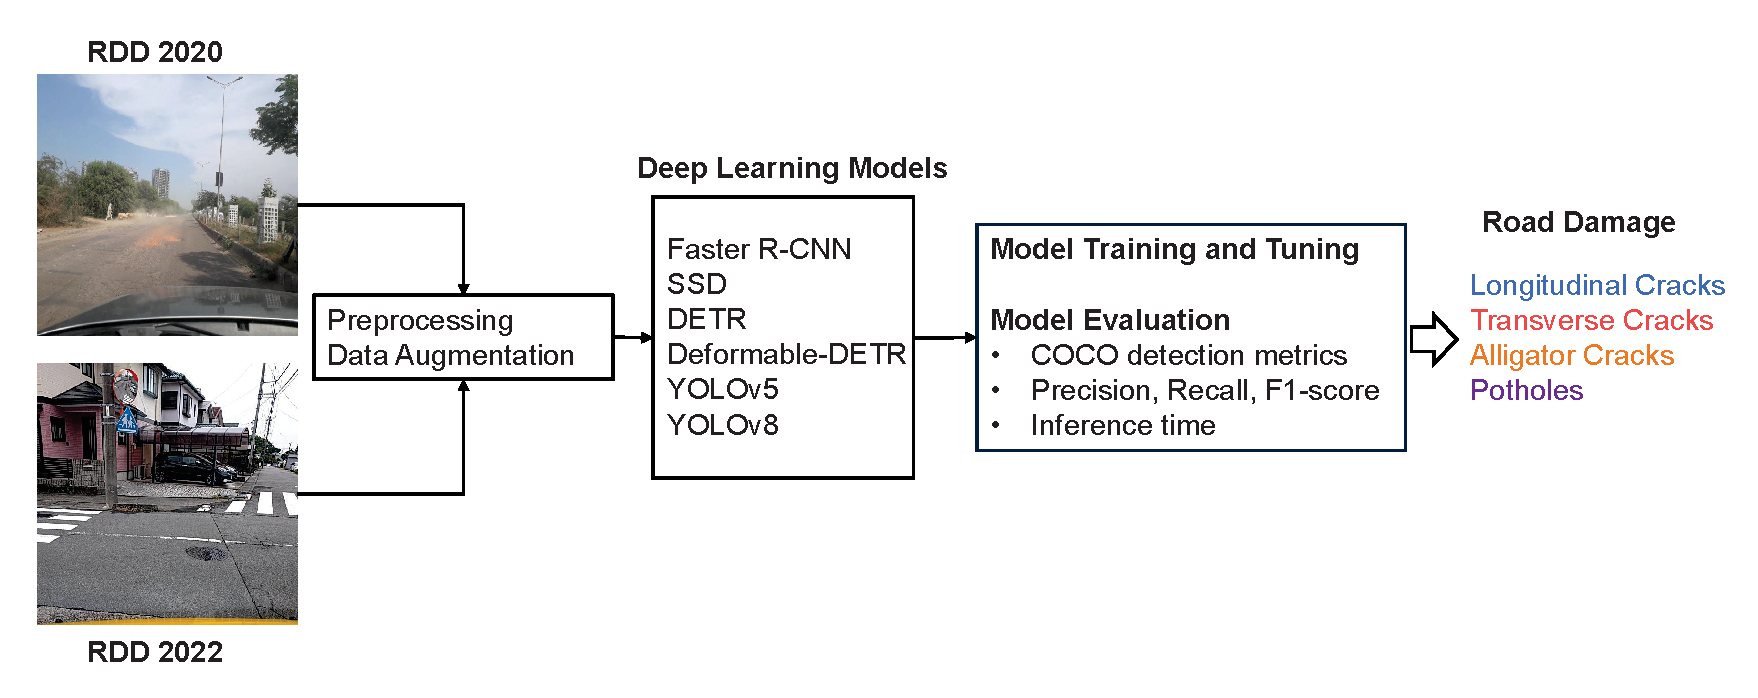
\includegraphics[width=0.9\textwidth]{figs/Figure_overview.eps}
    \caption{An overview of our automated road damage detection framework. We have considered two public datasets (RDD-2020 \cite{arya_grddc20} and RDD-2022 \cite{arya_rdd2022}. In this analysis, we have performed performance comparisons of six state-of-the-art deep learning models (Faster-RCNN \cite{ren_faster}, SSD with MobileNet backbone \cite{liu_ssd}, YOLOv5 \cite{yolo_v5}, YOLOv8, DETR \cite{carion_detr}, and Deformable DETR \cite{zhu_deformable_detr}). We use COCO detection metrics, precision, recall, F1 score, and inference times to elicit deeper insights and future research directions. In this work, we have considered four common types of damages (longitudinal cracks, transverse cracks, alligator cracks, and potholes).} \label{fig:overview}.
\end{figure*}

\subsection{Dataset}
The RDD-2022 dataset \cite{arya_rdd2022} has undergone significant changes over the years to improve its accuracy and extend its applicability to more countries. The original RDD-2018 dataset was introduced in 2018 \cite{maeda_rdd2018} and contained 9,053 road images with 15,435 instances of road damage. Later, the RDD-2018 dataset was used for the 2018 Road Damage Detection Challenge, in which 59 teams from 14 countries participated. However, the dataset was imbalanced, and suggestions were made to improve the annotation files. These suggestions were considered when RDD-2019 was introduced \cite{maeda_gan}, which corrected the annotations and augmented the dataset using generative adversarial networks (GAN). RDD-2019 included 13,133 images with 30,989 instances of road damage.

In 2020, an updated RDD-2020 dataset \cite{arya_grddc20} was introduced to extend the applicability of the models to more countries. The RDD-2020 dataset was formed by combining RDD-2019 with newly collected data from India and the Czech Republic. The RDD-2020 dataset included four damage categories: Longitudinal Cracks, Transverse Cracks, Alligator Cracks, and Potholes. The RDD-2020 dataset was used for the Global Road Damage Detection Challenge (GRDDC-2020), which invited researchers to propose a single model to monitor road conditions in India, Japan, and the Czech Republic with 21,041 images. The best-performing model achieved an F1 score of 0.67 using the YOLOv5-based ensemble model.

The RDD-2022 dataset has been introduced as part of the Crowd Sensing-based Road Damage Detection Challenge (CRDDC-2022) \cite{arya_rdd2022} to solve road damage detection for a more extensive set of countries, including India, Japan, the Czech Republic, Norway, China, and the United States with a total of 38,385 images released for the public. See Table \ref{tab:datasets} for more details on the RDD-2020 and RDD-2022 datasets. 

\begin{table*}[!ht]
\centering
\caption{Details of two public datasets (RDD-2020 \cite{arya_grddc20} and RDD-2022 \cite{arya_rdd2022}) used in this study.}
\label{tab:datasets}
\renewcommand*{\arraystretch}{1.15}
\begin{threeparttable}
\scriptsize
\setlength{\tabcolsep}{3pt}
\begin{tabularx}{\textwidth}{>{\raggedright\arraybackslash}p{1.35cm}>{\raggedright\arraybackslash}p{2.2cm}>{\raggedright\arraybackslash}p{2.2cm}>{\raggedright\arraybackslash}p{1.5cm}>{\raggedright\arraybackslash}p{1cm}>{\raggedright\arraybackslash}p{1.8cm}>{\raggedright\arraybackslash}p{0.95cm}>{\raggedright\arraybackslash}p{0.95cm}>{\raggedright\arraybackslash}p{0.95cm}>{\raggedright\arraybackslash}p{0.95cm}>{\raggedright\arraybackslash}p{0.95cm}}
\hline \hline
Dataset & Countries & Devices & Vehicles & Images & Resolution & Labels & D00 & D10 & D20 & D40  \\ \hline
RDD 2020 & Japan, \newline India,  \newline Czech & Smartphones & Cars & 21,041 & 600 $\times$ 600,   \newline 720 $\times$ 720 & 25,046 & 6,592 & 4,446 & 8,381 & 5,627 \\ \hline
RDD 2022 & Japan,  \newline India,  \newline Czech,  \newline Norway,  \newline United States,  \newline China (drones),  \newline China (motorbikes) & Smartphones, \newline Cameras, \newline Google Street View images & Cars, \newline Motorbikes, \newline Drones & 38,385 & 512 $\times$ 512,  \newline 600 $\times$ 600, \newline 720 $\times$ 720,  \newline 3650 $\times$ 2044 & 55,007 & 26,016 & 11,830 & 10,617 & 6,544  \\ \hline \hline
\end{tabularx}%
\begin{tablenotes}
    \small{
    \item D00: longitudinal cracks; D10: transverse cracks; D20: alligator cracks; D40: potholes
    }
\end{tablenotes}
\end{threeparttable}
\end{table*}

\subsection{Data Preparation}
The RDD-2022 \cite{arya_rdd2022} dataset is in PASCAL VOC format\footnote{http://host.robots.ox.ac.uk/pascal/VOC/}. However, to make it more compatible with the latest object detection techniques, we converted the annotations to the Common Objects in Context (COCO)\footnote{\url{https://cocodataset.org/\#home}} format. To focus on the specific types of road damage that are of particular interest, images from four damage classes were selected and filtered from the dataset. The four damage classes include longitudinal cracks (D00), transverse cracks (D10), alligator cracks (D20), and potholes (D40). 

It is essential to ensure that a deep learning model is trained on a diverse set of images and can generalize well to new, unseen data. To prepare the data for training and testing, a train-test split was performed. This involved random selection of 10\% of the data available from each country as a holdout set (test). The remaining data were split 90:10 for training and validation while maintaining class balance. 
%During modeling training, it was discovered that the choice of data used in the train-test split was critical.
%The model performed poorly when the data were split country-wise, likely due to poor generalizability. Therefore, it was essential to balance the data selection to ensure the model could generalize well to new, unseen data from different countries. 

\subsection{Detection Architectures}

The experiments tested the performance of four different deep-learning network architectures for object detection. These architectures were Faster-RCNN \cite{ren_faster}, SSD with MobileNet backbone \cite{liu_ssd}, YOLOv5 \cite{yolo_v5}, YOLOv8, DETR \cite{carion_detr}, and Deformable DETR \cite{zhu_deformable_detr}. The architectures are briefly described as follows:


\textbf{Faster R-CNN} \cite{ren_faster} architecture is a popular choice for object detection tasks. It consists of two main components: a region proposal network (RPN) and a detection network. The RPN generates candidate object regions that are then passed to the detection network for classification and regression of the bounding box. In our study of road damage detection using computer vision models, we chose the Faster R-CNN architecture with an RPN based on the ResNet50-FPN (Feature Pyramid Network) backbone. ResNet50-FPN combines the ResNet50 architecture with a feature pyramid module \cite{fpn_lin} to effectively capture multi-scale features. This choice enables accurate object localization and improves the model's ability to handle variations in road damage instances. Faster R-CNN with ResNet50-FPN has been widely adopted in various computer vision applications and offers a strong foundation for our road damage detection study.

\textbf{Single Shot MultiBox Detector (SSD)-MobileNet} \cite{liu_ssd} is a single-stage CNN architecture to achieve high detection accuracy with real-time processing speed. For our study on road damage detection using computer vision models, we employ SSD-MobileNet, where MobileNet serves as the base network for feature extraction. We used MobileNetv3 \cite{mobilenetv3_howard} for our implementation, a lightweight convolutional neural network architecture designed for mobile and embedded vision applications. SSD-MobileNet applies convolutional layers of different scales to capture objects at multiple resolutions. Each layer predicts a set of bounding boxes and class probabilities at different scales, resulting in a multi-scale feature map.

% \subsubsection{YOLO-Based Detectors}
\textbf{YOLOv5.} YOLO detectors \cite{redmon_yolo} have played an essential role in advancing object detection techniques. They employ a unique architecture that combines high detection accuracy with real-time inference speed. The original YOLO architecture revolutionized object detection by introducing a single-stage approach that directly predicts bounding boxes and class probabilities using a unified neural network. This eliminated the need for region proposal networks and postprocessing steps, resulting in faster inference times. Over time, several iterations and improvements have been made to the YOLO architecture, leading to the development of different versions of the YOLO model. YOLOv5 \cite{yolo_v5} is a notable advancement in the YOLO series. It consists of convolutional layers followed by upsampling and concatenation operations. YOLOv5 employs anchor boxes and predicts bounding box offsets and objectness scores for each anchor. It has gained popularity because of its simplicity, speed, and competitive performance on various object detection benchmarks. YOLOv5 offers a trade-off between accuracy and efficiency, making it well-suited for real-time road damage detection tasks. We use YOLOv5X in this work.

\textbf{YOLOv8} is an extension of the YOLOv5 architecture based on advances in network design and training strategies. It introduces the  (Coarse to fine) module, which replaces CSPLayer (Cross Stage Partial), effectively combining high-level features with contextual information to improve detection accuracy. Using an anchor-free model with a decoupled head, YOLOv8 allows independent processing of objectness, classification, and regression tasks, improving overall accuracy. The YOLOv8 output layer adopts the sigmoid activation function for the objectness score, indicating the probability of a bounding box containing an object. In contrast, class probabilities are computed using the softmax function.

Furthermore, YOLOv8 incorporates the CIoU (Complete Intersection over Union) and DFL (Distribution Focal Loss) loss functions for bounding-box loss, enabling better performance detecting smaller objects and employing binary cross-entropy for classification loss. With its real-time processing speed and enhanced detection capabilities, YOLOv8 proves to be a promising choice for real-time road damage detection tasks that prioritize both accuracy and efficiency. We use YOLOv8X in this work.

% \subsubsection{Detection Transformers}
\textbf{Detection Transformer} (DETR) \cite{carion_detr} is a recent object detection architecture that replaces traditional two-stage detectors with a transformer-based framework. It models object detection as a direct set prediction problem, where a convolutional backbone processes the input image, and a transformer encoder-decoder architecture generates the final set of bounding box predictions and class probabilities. DETR benefits from the attention mechanism of transformers, which allows it to capture global dependencies between objects efficiently. It has shown promising results in object detection tasks and offers potential advantages for road damage detection by leveraging its ability to handle complex spatial relationships between damage instances.

\textbf{Deformable-DETR} \cite{zhu_deformable_detr} is an extension of DETR incorporating deformable convolutional layers. Deformable convolutions allow the network to adaptively adjust the sampling locations of convolutional kernels, enabling better modeling of geometric variations in objects. Integrating deformable convolutions and multi-scale features into the DETR architecture, Deformable-DETR improves the localization accuracy and robustness of object detection while reducing computational complexity and training convergence times. This makes it well suited for road damage detection, where precise localization of damage instances is crucial.

\begin{table*}[!t] 
\centering  
\renewcommand*{\arraystretch}{1.2}
\caption{Object detection models implemented and evaluated in this work, including optimization algorithms, loss functions, and hyperparameter settings.}
\label{table:models}
\begin{threeparttable}
\scriptsize
\setlength{\tabcolsep}{4pt}
\begin{tabularx}{\textwidth}{>{\raggedright\arraybackslash}p{1.8cm}>{\raggedright\arraybackslash}X>{\centering\arraybackslash}p{1.2cm}>{\raggedright\arraybackslash}p{1.7cm}>{\raggedright\arraybackslash}p{1.4cm}>{\centering\arraybackslash}p{0.9cm}>{\centering\arraybackslash}p{0.9cm}>{\centering\arraybackslash}p{1.05cm}}
\toprule
\textbf{Model} & \textbf{Description} & \textbf{Optimizer} & \textbf{Loss Function} & \textbf{Augmentation} & \textbf{LR} & \textbf{Epochs}& \textbf{Batch Size}\\
\midrule
Faster R-CNN \cite{ren_faster}  & ImageNet \cite{imagenet_deng} pre-trained ResNet50-FPN backbone with Faster-RCNN detection head & SGD & Classification + Localization loss & Horizontal flips & 0.0001 & 30 & 4 \\
SSD-MobileNet \cite{liu_ssd} & ImageNet \cite{imagenet_deng} pre-trained MobileNet-v3-large backbone with single-shot detector & SGD & Classification + Localization + Objectness loss & Flips + crops & 0.001 & 300 & 4 \\
YOLOv5X \cite{yolo_v5} & Modified YOLO architecture with CSPDarkNet53 backbone & Adam & Compound loss & Various & 0.001 & 30 & 16 \\
YOLOv8X \cite{yolov8} & Extension of YOLOv5, introduces C2f module & Adam & CIoU + DFL loss & Advanced & 0.001 & 100 & 16 \\
DETR \cite{carion_detr}  & Detection Transformer with ResNet50 CNN backbone for feature extraction & AdamW & Set loss & Standard & $1\times10^{-5}$ & 300 & 16 \\
Deformable DETR \cite{zhu_deformable_detr} & Extension of DETR with deformable convolution layers & AdamW & Set loss & Standard & $2\times10^{-4}$ & 50 & 4 \\
\bottomrule
\end{tabularx}
\begin{tablenotes}
    \small {
    \item{SGD: Stochastic Gradient Descent}
    \item CIoU: Complete intersection over union
    \item DFL: Distribution Focal Loss
    \item C2f: Cross-Stage Partial bottleneck with two convolutions}
\end{tablenotes}
\end{threeparttable}
\end{table*}

\subsection{Implementation Details}
The Faster R-CNN and SSD models were implemented using the PyTorch deep learning framework. DETR and Deformable-DETR models (based on the transformer architecture) were implemented using the original PyTorch implementations (PyTorch 2.0, Python 3.9, CUDA 11.7). YOLO-based models (YOLOv5X and YOLOv8X) were implemented using the ultralytics\footnote{https://github.com/ultralytics} framework. All models were trained on a high-performance computing (HPC) cluster featuring Nvidia A100 GPUs, and a single A100 GPU was placed in a Linux environment (Red Hat Enterprise 9 based on Fedora).

The details of the training process for each model, including optimization algorithms, loss functions, and hyperparameter settings, are summarized in Table \ref{table:models}. This table provides an overview of the learning rate, batch size, number of epochs, and other vital parameters used during training for each model architecture. 


Model evaluation is a critical step in assessing the performance and effectiveness of object detection models. In this subsection, we discuss the performance metrics used to evaluate the models and the evaluation protocols followed for the evaluation.

\subsubsection{Evaluation Metrics}
\label{sec:metrics}

During the evaluation of object detection models, various metrics are commonly used to assess their performance rigorously. These metrics provide valuable information on different aspects of model performance, including precision, recall, average precision, and the trade-off between precision and recall. The following evaluation metrics were utilized in our analysis:

\begin{enumerate}
  \item \textbf{Intersection over Union (IoU):} The IoU metric measures the overlap between the predicted bounding boxes and the ground truth boxes, indicating the accuracy of object localization. It is calculated using the following formula:
  
  \[IoU = \frac{\text{Area of Intersection}}{\text{Area of Union}}\]
  
  \item \textbf{Precision:} Precision denotes the proportion of true positive detections out of all positive detections made by the model. It quantifies the accuracy of the model's predictions and is calculated as follows:
  
  \[Precision = \frac{\text{True Positives}}{\text{True Positives + False Positives}}\]
  
  \item \textbf{Recall:} Recall measures the proportion of true positive detections out of all ground-truth positive instances. It reflects the model's ability to find all relevant objects and is calculated as,   
  \[Recall = \frac{\text{True Positives}}{\text{True Positives + False Negatives}}\]
  
  \item \textbf{F1 Score:} The F1 score is the harmonic mean of precision and recall, providing a single metric to assess the overall performance of the model. It is given by:  
  \[\text{\textit{F1 Score}} = 2 \times \frac{\text{Precision} \times \text{Recall}}{\text{Precision + Recall}}\]

  \item \textbf{Average Precision (AP):} The AP metric quantifies the performance of object detection by measuring the area under the precision-recall curve. It considers the precision values at various recall levels and calculates their average, providing an overall assessment of the model's detection accuracy for a specific IoU threshold.

  \item \textbf{Mean Average Precision (mAP):} The mAP is a widely used metric that calculates the average precision in different IoU thresholds. It provides an overall assessment of the model's performance. The mAP is computed as the mean of the average precision (AP) values obtained at various IoU thresholds.
  
  \item \textbf{COCO-style AP (AP@[IoU thresholds] - [Size categories]):} The COCO-style AP assesses the average precision at predefined IoU thresholds specified by the COCO dataset. It gauges the model's performance across various IoU values, such as 0.5, 0.75, and 0.95, while considering object size categories: small, medium, and large. This metric provides insights into the model's detection accuracy across different object scales and levels of overlap.
  
  \item \textbf{COCO-style AR (AR@[max detections] - [size categories]):} The COCO-style AR metric evaluates average recall at different maximum detections per image, following the definitions of the COCO dataset. It considers the model's object detection performance across different scenarios of top detections per image, considering object size categories: small, medium, and large. This metric provides insights into the model's capability to detect objects under diverse conditions of detection output.
\end{enumerate}

In addition to these evaluation metrics, precision-recall curves are commonly utilized to analyze the model's performance across different confidence thresholds. These curves plot precision against recall, enabling a comprehensive assessment of the precision-recall trade-off and performance characteristics of the object detection models.

\subsubsection{Evaluation Protocol}
During model evaluation, the designated test set is used to evaluate the performance of the models. The test set consists of labeled images with annotated ground-truth bounding boxes, allowing for the comparison of predicted bounding boxes against the ground truth.

To evaluate the models, the following protocol was followed:
\begin{enumerate}[noitemsep,topsep=0pt]
    \item \textit{Input images:} The test set images were fed into the object detection models, and the bounding box predictions were generated for the objects in the images.
    \item \textit{Calculation of the intersection over the union (IoU):} The IoU was calculated between the predicted bounding boxes and the corresponding ground truth boxes to determine the accuracy of object localization.
    \item \textit{Evaluation metrics:} Using IoU values, metrics such as precision, recall, average precision (AP), F1 score, mean average precision (mAP), COCO-style AP and COCO-style AR were calculated to evaluate model performance.
    \item \textit{Precision recall curve:} By varying confidence thresholds, precision and recall values were obtained, which were then used to plot the precision-recall curve.
    \item \textit{Comparative analysis:} Evaluation metrics and precision-recall curves were analyzed to compare the performance of different object detection models and identify the strengths and weaknesses of each approach.
\end{enumerate}


\section{Results and discussion}
In this section, we provide both quantitative and qualitative results.

\subsection{Quantitative Results}
Road damage detection models were evaluated by comparing their performance using object detection metrics, as detailed in Section \ref{sec:metrics}. This evaluation was conducted on the test sets derived from the RDD-2020 and RDD-2022 datasets. Table \ref{tab:results_coco} provides a comprehensive summary of the COCO object detection metrics achieved by the various models in the RDD-2020 and RDD-2022 datasets.

\begin{table*}[!ht]
\caption{Comparison of performance of six state-of-the-art models on RDD-2020 \cite{arya_grddc20} and RDD-2022 \cite{arya_rdd2022} datasets using COCO detection metrics.}
\centering
\label{tab:results_coco}
\begin{adjustbox}{max width=\textwidth}
\begin{threeparttable}
\scriptsize
\setlength{\tabcolsep}{3pt}

\begin{tabular}{@{}lcccccccccccc@{}}
\toprule
Model/Metric    & AP    & AP    & AP    & AP    & AP    & AP    & AR    & AR    & AR    & AR    & AR    & AR \\
                & 0.50  & 0.50  & 0.75  & 0.50  & 0.50  & 0.50  & 0.50  & 0.50  & 0.50  & 0.50  & 0.50  & 0.50 \\
IoU Threshold   & :0.95 &       &       & :0.95 & :0.95 & :0.95 & :0.95 & :0.95 & :0.95 & :0.95 & :0.95 & :0.95 \\
\midrule
MaxDets         & 100   & 100   & 100   & 100   & 100   & 100   & 1     & 10    & 100   & 100   & 100   & 100   \\
\midrule
Area            & all   & all   & all   & small & medium& large & all   & all   & all   & small & medium & large \\
\midrule
 & \multicolumn{12}{c}{Results on the RDD-2020 \cite{arya_grddc20} dataset} \\
\midrule
Faster R-CNN \cite{ren_faster}     & 0.157 & 0.386 & 0.096 & 0.099 & 0.116 & 0.191 & 0.205 & 0.372 & 0.388 & 0.244 & 0.350 & 0.440 \\
SSD \cite{liu_ssd}            & 0.078 & 0.183 & 0.051 & 0.002 & 0.035 & 0.126 & 0.137 & 0.247 & 0.309 & 0.062 & 0.222 & 0.425 \\
DETR \cite{carion_detr}            & 0.197 & 0.452 & 0.148 & 0.116 & 0.139 & 0.251 & 0.239 & 0.428 & 0.524 & 0.295 & 0.473 & \textbf{0.614} \\
Deformable-DETR \cite{zhu_deformable_detr} & 0.197 & 0.460 & 0.142 & 0.127 & 0.146 & \textbf{0.260}  & \textbf{0.256} & 0.438 & 0.484 & 0.307 & 0.439 & 0.574 \\
YOLOv5X \cite{yolo_v5}  & 0.196 & 0.461 & 0.135 & 0.112 & 0.161 & 0.214 & 0.233 & 0.439 & 0.500 & 0.364 & 0.479 & 0.530 \\
YOLOv8X  \cite{yolov8}        & \textbf{0.223} & \textbf{0.488} & \textbf{0.169} & \textbf{0.141} & \textbf{0.177} & 0.253 & 0.25  & \textbf{0.473} & \textbf{0.536} & \textbf{0.423} & \textbf{0.510} & 0.575 \\
\midrule
 & \multicolumn{12}{c}{Results on the RDD-2022 \cite{arya_rdd2022} dataset} \\
\midrule
Faster R-CNN \cite{ren_faster}      & 0.211 & 0.478 & 0.156 & 0.074 & 0.160 & 0.239 & 0.235 & 0.399 & 0.417 & 0.210 & 0.370 & 0.459 \\
SSD \cite{liu_ssd}              & 0.092 & 0.213 & 0.064 & 0.001 & 0.045 & 0.127 & 0.139 & 0.247 & 0.300 & 0.039 & 0.215 & 0.377 \\
DETR  \cite{carion_detr}          & 0.251 & 0.516 & 0.217 & 0.121 & 0.171 & 0.298 & 0.260 & 0.455 & 0.538 & 0.334 & 0.467 & \textbf{0.607} \\
Deformable-DETR \cite{zhu_deformable_detr} & 0.252 & 0.516 & 0.212 & \textbf{0.160} & 0.185 & 0.293 & 0.271 & 0.472 & 0.519 & 0.379 & 0.459 & 0.579 \\
YOLOv5X \cite{yolo_v5}         & 0.275 & \textbf{0.561} & 0.238 & 0.131 & \textbf{0.228} & 0.295 & 0.272 & 0.477 & 0.531 & \textbf{0.399} & 0.501 & 0.557 \\
YOLOv8X \cite{yolov8}         & \textbf{0.281} & 0.547 & \textbf{0.252} & 0.134 & \textbf{0.228} & \textbf{0.303} & \textbf{0.273} & \textbf{0.495} & \textbf{0.547} & 0.389 & \textbf{0.515} & 0.589 \\
\bottomrule
\end{tabular}
\begin{tablenotes}
    \small {
    \item{\textbf{AP}: Average Precision; \textbf{AR}: Average Recall} }
\end{tablenotes}
\end{threeparttable}
\end{adjustbox}
\end{table*}

As seen in Table \ref{tab:results_coco}, a notable performance improvement is evident in all models when switching from the RDD-2020 \cite{arya_grddc20} to the RDD-2022 \cite{arya_rdd2022} datasets. This performance improvement can be attributed to the infusion of additional data from various countries into the RDD-2022 dataset. This underscores the important role of rich and diverse data in improving model performance. Across both the RDD-2020 \cite{arya_grddc20} and RDD-2022 \cite{arya_rdd2022} datasets, YOLOv8 consistently demonstrated superior performance compared to other models, which is reflected in its higher average precision and average recall metrics across different thresholds. The YOLOv5 \cite{yolo_v5}, Deformable-DETR \cite{zhu_deformable_detr}, and DETR \cite{carion_detr} models also closely trail the YOLOv8 model \cite{yolov8} in terms of performance. On the contrary, SSD \cite{liu_ssd} (the most compact model) exhibited sub-par performance in all metrics. This indicates the demand for greater capacity of the model to capture intricate patterns of road damage effectively.

When assessing the performance of road damage detection in various dimensions and scales, a general trend observed is that all models demonstrate respectable performance with larger dimensions of the bounding box, which gradually decreases as smaller sizes are introduced. On this note, the Deformable-DETR model \cite{zhu_deformable_detr} employs deformable convolutions to enhance the detection of more minor damages. On closer inspection of the results, the Deformable-DETR model exhibits significantly better performance with smaller dimensions when compared to other models. However, this advantage does not extend to larger bounding boxes, which reveals a limitation of this model. A slight but notable performance improvement is also observed with the updated YOLOv8 model compared to the YOLOv5 \cite{yolo_v5} model. Although both models exhibit strong performance, the YOLOv8 model \cite{yolov8}  has slightly better performance due to the more efficient architecture. 

Compared with different IoU thresholds for evaluation, the general trend is that the models decrease precision and recall values with increasing IoU thresholds. However, the YOLOv8 model \cite{yolov8} is more tolerant to higher IoU thresholds and maintains a more balanced result across different IoU thresholds. For recall values, both the DETR \cite{carion_detr} and Deformable-DETR \cite{zhu_deformable_detr} models have a higher recall compared to their precision, suggesting that these models are more likely to detect objects but might have more false positives. The YOLOv8 architecture \cite{yolov8}, despite having the highest precision, maintains consistent recall values, making it a more balanced choice. In general, YOLOv8 seems to be the model that performs best, with YOLOv5 \cite{yolo_v5}, Deformable-DETR \cite{zhu_deformable_detr}, and DETR \cite{carion_detr} closely following.

\begin{table*}[!ht]
\centering
\caption{Comparison of performance of six state-of-the-art models for four crack classes. The four road damage classes are longitudinal cracks (D00), transverse cracks (D10), alligator cracks (D20), and potholes (D40). The best results are highlighted in bold text.}
\label{tab:classwise}
\begin{threeparttable}
\begin{tabular}{m{0.1\textwidth}m{0.1\textwidth}m{0.1\textwidth}m{0.1\textwidth}m{0.1\textwidth}m{0.1\textwidth}m{0.1\textwidth}m{0.1\textwidth}}
\toprule
& \multicolumn{7}{c}{Models} \\  % Adjust column header
\cmidrule(l){3-8}

\multirow{2}{*}{\parbox{0.1\textwidth}{Damage Category}} & 
\multirow{2}{*}{\parbox{0.1\textwidth}{Metric}} &
\multirow{2}{*}{\parbox{0.1\textwidth}{Faster-RCNN}} &
\multirow{2}{*}{\parbox{0.1\textwidth}{SSD}} &
\multirow{2}{*}{\parbox{0.1\textwidth}{DETR}} &
\multirow{2}{*}{\parbox{0.1\textwidth}{Deformable DETR}} &
\multirow{2}{*}{\parbox{0.1\textwidth}{YOLOv5X}} &
\multirow{2}{*}{\parbox{0.1\textwidth}{YOLOv8X}}  \\ \\

\midrule
\multicolumn{8}{c}{Results on the RDD-2020 \cite{arya_grddc20} dataset} \\
\midrule
\multirow{4}{*}{D00}
& Precision & 0.3874 & 0.1998 & 0.4058 & 0.4638 & 0.4504 & \textbf{0.4945} \\
& Recall & 0.3947 & 0.2730 & \textbf{0.4774} & 0.4399 & 0.4743 & 0.4212 \\
& F1 Score & 0.3910 & 0.2307 & 0.4387 & 0.4516 & \textbf{0.4620} & 0.4549 \\
& AP & 0.3183 & 0.1420 & 0.3688 & 0.3767 & \textbf{0.4017} & 0.3851 \\
\midrule
\multirow{4}{*}{D10}
& Precision & 0.4186 & 0.1781 & 0.4877 & 0.4555 & 0.4734 & \textbf{0.4911}\\
& Recall & 0.3682 & 0.1955 & 0.4523 & 0.5000 & 0.4455 & \textbf{0.5023} \\
& F1 Score & 0.3918 & 0.1863 & 0.4693 & 0.4767 & 0.4590 & \textbf{0.4966} \\
& AP & 0.3315 & 0.0874 & 0.4101 & 0.4182 & 0.4105 & \textbf{0.4411} \\
\midrule
\multirow{4}{*}{D20}
& Precision & 0.5898 & 0.5540 & 0.5943 & 0.6278 & 0.6443 & \textbf{0.6389} \\
& Recall & 0.5337 & 0.3975 & \textbf{0.6462} & 0.6050 & 0.5750 & 0.6238 \\
& F1 Score & 0.5604 & 0.4629 & 0.6192 & 0.6162 & 0.6077 & \textbf{0.6312} \\
& AP & 0.5542 & 0.4156 & 0.6188 & 0.6047 & 0.6033 & \textbf{0.6613} \\
\midrule
\multirow{4}{*}{D40}
& Precision & 0.3866 & 0.1532 & 0.5113 & 0.5310 & 0.4281 & \textbf{0.5683} \\
& Recall & 0.3797 & 0.1390 & 0.4029 & 0.4421 & \textbf{0.4724} & 0.4153 \\
& F1 Score & 0.3831 & 0.1458 & 0.4506 & 0.4825 & 0.4492 & \textbf{0.4799} \\
& AP & 0.3139 & 0.0550 & 0.3879 & 0.4227 & 0.4094 & \textbf{0.4464} \\
\midrule
\multicolumn{8}{c}{Results on the RDD-2022 \cite{arya_rdd2022} dataset} \\
\midrule
\multirow{4}{*}{D00}
& Precision & 0.5679 & 0.3347 & 0.5665 & 0.5554 & 0.5820 & \textbf{0.6132} \\
& Recall & 0.4906 & 0.2556 & 0.5044 & 0.5288 & \textbf{0.5682} & 0.5010 \\
& F1 Score & 0.5264 & 0.2899 & 0.5337 & 0.5418 & \textbf{0.5750} & 0.5514 \\
& AP & 0.4929 & 0.1999 & 0.4998 & 0.5048 & \textbf{0.5518} & 0.5258 \\
\midrule
\multirow{4}{*}{D10}
& Precision & 0.5415 & 0.3239 & 0.5787 & 0.5767 & 0.6176 & \textbf{0.6691} \\
& Recall & 0.4799 & 0.2995 & 0.5569 & 0.5298 & 0.5333 & \textbf{0.5595} \\
& F1 Score & 0.5088 & 0.3112 & 0.5676 & 0.5523 & 0.5724 & \textbf{0.6094} \\
& AP & 0.4864 & 0.1942 & 0.5497 & 0.5515 & 0.5605 & \textbf{0.5891} \\
\midrule
\multirow{4}{*}{D20}
& Precision & 0.5946 & 0.5622 & 0.6748 & 0.6071 & 0.6436 & \textbf{0.7051} \\
& Recall & 0.5690 & 0.3937 & 0.5862 & \textbf{0.6054} & \textbf{0.6054} & 0.5450 \\
& F1 Score & 0.5815 & 0.4631 & \textbf{0.6274} & 0.6062 & 0.6239 & 0.6148 \\
& AP & 0.5909 & 0.4060 & 0.6323 & 0.6015 & \textbf{0.6404} & 0.6383 \\
\midrule
\multirow{4}{*}{D40}
& Precision & 0.4184 & 0.0849 & 0.4454 & 0.4462 & \textbf{0.5804} & 0.5009 \\
& Recall & 0.3760 & 0.1654 & 0.4009 & \textbf{0.4727} & 0.4446 & 0.4462 \\
& F1 Score & 0.3961 & 0.1122 & 0.4220 & 0.4591 & \textbf{0.5035} & 0.4719 \\
& AP & 0.3272 & 0.0306 & 0.3746 & 0.3957 & \textbf{0.4839} & 0.4286 \\
\bottomrule
\end{tabular}
\begin{tablenotes}
    \small{
    \item AP: Average Precision
    \item D00: longitudinal cracks; D10: transverse cracks; D20: alligator cracks; D40: potholes
    } 
\end{tablenotes}
\end{threeparttable}
\end{table*}

\begin{figure*}[!ht] % 
    \centering 
    \includegraphics[width=0.75\textwidth]{figs/prc_classwise_rdd20.pdf} % Adjust width as needed
    \caption{Precision-Recall curves for the best performing models (DETR \cite{carion_detr}, Deformable DETR \cite{zhu_deformable_detr}, YOLOv5 \cite{yolo_v5} and YOLOv8 \cite{yolov8}) on the RDD-2020 \cite{arya_grddc20} dataset. The best results are highlighted in bold text.}
    \label{fig:prc_rdd20}
\end{figure*}

\begin{figure*}[!ht] % 
    \centering 
    \includegraphics[width=0.75\textwidth]{figs/prc_classwise_rdd22.pdf} % Adjust width as needed
    \caption{Precision-Recall curves for the best performing models (DETR \cite{carion_detr}, Deformable DETR \cite{zhu_deformable_detr}, YOLOv5 \cite{yolo_v5} and YOLOv8 \cite{yolov8}) on the RDD-2022 \cite{arya_rdd2022} dataset.}
    \label{fig:prc_rdd22}
\end{figure*}

Table \ref{tab:classwise} presents the class-wise performance of six state-of-the-art models for the RDD-2020 \cite{arya_grddc20} and RDD-2022 \cite{arya_rdd2022} datasets. We notice trends similar to those observed in the COCO object detection metrics presented in Table \ref{tab:results_coco}, where the introduction to the RDD-2022 \cite{arya_rdd2022} dataset leads to an improvement in the detection scores across the board. Models based on the YOLO architecture exhibit notable performance, leading several class-wise detection metrics. The YOLOv8 model \cite{yolov8} shows the best performance in the RDD-2020 dataset \cite{arya_grddc20} and also shows competitive performance across different classes of the RDD-2022 dataset. Interestingly, despite the advantage of YOLOv8 in COCO mAP metrics (as shown in Table \ref{tab:results_coco}), the YOLOv5 model \cite{yolo_v5} offers better performance in three of the four damage categories within the RDD-2022 dataset. This discrepancy highlights the effect of the class imbalance of the datasets. 

When we look at the difference in performance across various classes, all models tend to have higher precision and an F1 score for the ``D20" damage category (alligator cracks). On visual examination of these cracks, their relatively larger size and distinct features are evident, making them easy to detect by the models. On the contrary, the ``D40" damage category (potholes) is, in general, not only smaller in dimensions but also has fewer samples in the datasets. The limited representation likely poses additional challenges to the models' difficulties in detection, as evidenced by the performance metrics. Regarding the remaining two damage categories, ``D00" (longitudinal cracks) and ``D10" (transverse cracks), all models show comparable performance metrics that align with their similarity in visual characteristics. 

The DETR models exhibit commendable performance in various damage categories, although they slightly trail behind the YOLO models. The introduction to deformable convolution yields exciting results. This architectural tweak improves performance on longitudinal and transverse cracks, as well as potholes while resulting in a performance drop for alligator cracks. This reveals a nuanced impact of architectural changes and also underscores the limitation of Deformable-DETR \cite{zhu_deformable_detr} in the detection of larger cracks. In general, DETR-based models \cite{carion_detr, zhu_deformable_detr} demonstrate strong performance in most damage categories. However, compared to the YOLO models \cite{yolo_v5, yolov8}, they show diminished performance in pothole detection. 

In summary, except SSD \cite{liu_ssd}, all models demonstrate competitive performance in various performance metrics for detecting road damage. The performance of more advanced models based on DETR \cite{carion_detr, zhu_deformable_detr} or YOLO \cite{yolo_v5, yolov8} architectures is particularly notable. Both YOLO models demonstrate versatility and robustness in effectively addressing various crack types.

\subsubsection*{Precision-Recall Curves}

Figures \ref{fig:prc_rdd20} and \ref{fig:prc_rdd22} visually represent the precision-recall curves for the different damage categories within the RDD-2022 \cite{arya_rdd2022} dataset, highlighting the performance of the best performing models (DETR \cite{carion_detr}, Deformable DETR \cite{zhu_deformable_detr}, YOLOv5 \cite{yolo_v5} and YOLOv8 \cite{yolov8}). Depending on the damage category, all models tend to follow a general trend for the precision-recall curves. The precision-recall curves corroborate the insights from Table \ref{tab:classwise}, with the YOLOv5 and YOLOv8 models leading in performance.  

\subsubsection{Confusion Matrices}
\begin{figure*}[!ht] % 
    \centering 
    \includegraphics[width=0.75\textwidth]{figs/confusion_matrix_rdd20.pdf}
    \caption{Normalized confusion matrices, comparing performances of best-performing models (DETR \cite{carion_detr}, Deformable DETR \cite{zhu_deformable_detr}, YOLOv5 \cite{yolo_v5} and YOLOv8 \cite{yolov8}) on the RDD-2020 dataset.}
    \label{fig:conf_rdd20}
\end{figure*}

\begin{figure*}[!ht] %  
    \centering 
    \includegraphics[width=0.75\textwidth]{figs/confusion_matrix_rdd22.pdf}
    \caption{Normalized confusion matrices, comparing performances of best-performing models (DETR \cite{carion_detr}, Deformable DETR \cite{zhu_deformable_detr}, YOLOv5 \cite{yolo_v5} and YOLOv8 \cite{yolov8}) in the RDD-2022 \cite{arya_rdd2022} dataset.}
    \label{fig:conf_rdd22}
\end{figure*}

Confusion matrices were computed for various models using the RDD-2020 \cite{arya_grddc20} and RDD-2022 \cite{arya_rdd2022} datasets. Normalized confusion matrices for the RDD-2020 and RDD-2022 datasets are illustrated in figures \ref{fig:conf_rdd20} and \ref{fig:conf_rdd22}, respectively. A close examination of the confusion matrices shows some interesting patterns, especially in contrast to the class-wise performance metrics documented in Table \ref{tab:classwise}. It is worth mentioning that a global confidence threshold was employed during the computation of the confusion matrices. This approach yields more overarching findings in diverse classes. 

\begin{table*}[!ht]
    \centering
    \caption{Comparison of state-of-the-art models used in this study and their inference time. The best result is highlighted in bold text.}
    \begin{tabular}{lccc}
        \toprule
         \textbf{Model} & \textbf{Input image size} & \textbf{Total model parameters} & \textbf{Average inference time (ms)}\\
         \midrule
         Faster R-CNN & 720 x 720 & 41.3 M & 15.10 \\
         SSD & 720 x 720 & 3.7 M & 8.84 \\
         DETR & 1200 x 800 & 41.5 M & 8.13 \\
         Deformable DETR &  1200 x 800 & 41 M & 22.58 \\
         YOLOv5X & 640 x 640 & 86.1 M & 6.32 \\
         YOLOv8X & 640 x 640 & 68.2 M & \textbf{5.91} \\
         \bottomrule
    \end{tabular}

    \label{tab:inference_time}
\end{table*}

Analyzing the confusion matrices of the RDD-2020 dataset \cite{arya_grddc20}, Deformable-DETR \cite{zhu_deformable_detr} is regarded as the best performer in terms of precision, closely followed by the results of the DETR architecture. However, the YOLOv5 \cite{yolo_v5} and YOLOv8 \cite{yolov8} architectures exhibit vulnerabilities in the detection of inevitable cracks, with the former demonstrating suboptimal performance in the detection of transverse cracks and the latter in the detection of potholes. Turning our attention to the RDD-2022 \cite{arya_rdd2022} dataset, the YOLOv5 \cite{yolo_v5} architecture shows a balanced overall performance. The Deformable-DETR architecture also remains competitive. The DETR \cite{carion_detr} and YOLOv8 architectures perform well in most damage categories, except potholes. 



Across both datasets, a recurring observation is that all models show some weakness in detecting pothole examination. They exhibit strong performance when detecting alligator cracks. The detection precision for longitudinal and transverse cracks is also commendable, with a few exceptions. Considering false positives, a uniform representation of the different damage categories is present for the RDD-2020 \cite{arya_grddc20} dataset. In contrast, the RDD-2022 \cite{arya_rdd2022} dataset is characterized by a rise in false positives for longitudinal cracks, leaving other damage categories with considerably lower false positive rates. Regarding false negatives, potholes consistently register the highest rates, underscoring the challenge of classifying this type of damage. 

A particularly salient observation from both confusion matrices is the models' remarkably low inter-class confusion. In other words, misclassifications across different damage categories are notably rare. This underscores the strengths of the models in distinguishing among types of damage. Our primary focus in the future would be to address and reduce the occurrence of false positives and false negatives. 

\subsection{Inference time}
Table \ref{tab:inference_time} compares the inference times of six state-of-the-art object detection models. Table \ref{tab:inference_time} also provides the input image size of the models and the corresponding number of model parameters. We can see that YOLOv8X has the least inference time (5.91 ms), which is highly suitable for real-time applications, such as road damage detection. We also observe that YOLOv5X is the second best, with an inference time of 6.32 ms.% In a general pattern, we see that the more complex the model is, the more parameters it will have and, therefore, the higher the inference time. For example, the Deformable DETR model is more complex and has a higher inference time (22.58 ms). The exception to this observation is the YOLO family models, which, despite having a more significant number of parameters, their inference times are lower. 
In general, a more complex model equates to a longer inference time, as can be seen with the Deformable DETR. However, it should be noted that the Deformable DETR variant we employed here utilizes special techniques such as iterative bounding box refinement and two-stage detection, which is responsible for the higher inference time. A variant without these modifications should have lower inference times at the cost of performance. The YOLO models, which are purpose-built for real-time applications, on the other hand, have significantly lower inference times due to the simpler architecture despite having a higher parameter count.

\subsection{Qualitative Results}
This section presents a qualitative analysis of different road damage detection models through visual examination of the RDD-2022 \cite{arya_rdd2022} dataset. Since the RDD-2020 dataset is a subset of the RDD-2022 dataset \cite{arya_rdd2022}, the predictions in the RDD-2022 dataset inherently cover the road damage scenarios present in the RDD-2020 dataset. The purpose of this visual analysis is to provide insights into the strengths and limitations of different models' predictions, as well as to explore any discrepancies between the ground-truth annotations and forecasts of the models. A detailed visual examination of the different types of road damage present in the RDD-2020 and RDD-2022 datasets concerning the predictions of the top-performing deep learning models for road damage detection helps us understand the performance of the models conceiving different types of road damage, spatial distribution, and overall prediction precision. This qualitative evaluation complements the quantitative metrics presented earlier, enhancing understanding of the effectiveness of the models.

Figure \ref{fig:det_rdd22} illustrates the road damage predictions of the top performing models, namely DETR \cite{carion_detr}, Deformable DETR \cite{zhu_deformable_detr}, YOLOv5 \cite{yolo_v5}, and YOLOv8 \cite{yolov8}. In general, these models demonstrate strong performance in detecting road damage instances. However, there are isolated cases where specific models struggle to identify road damage. The models collectively exhibit the ability to detect various types of road damage, including longitudinal cracks, transverse cracks, alligator cracks, and potholes, with a notable degree of accuracy.

\begin{figure*}[!ht] % 
    \centering 
    \includegraphics[width=\textwidth]{figs/good-preds/China_Drone_000917.pdf}
    \includegraphics[width=\textwidth]{figs/good-preds/Japan_006122.pdf}
    \includegraphics[width=\textwidth]{figs/good-preds/Japan_009915.pdf}
    \includegraphics[width=\textwidth]{figs/good-preds/United_States_001436.pdf}    
    \caption{\textbf{Road damage predictions} by four best models on the RDD-2022 \cite{arya_rdd2022} dataset. In the figure, each row corresponds to a sample of ground truth damages followed by predictions of DETR \cite{carion_detr}, Deformable DETR \cite{zhu_deformable_detr}, YOLOv5X \cite{yolo_v5} and YOLOv8X \cite{yolov8}.}
    \label{fig:det_rdd22}
\end{figure*}

While investigating the performance of the different models, we encountered an intriguing phenomenon in the behavior of the models, where we observed a considerably high number of false positives, which impacted the overall detection scores. A meticulous examination of the predictions revealed certain cases where the models detected road damages that were not present in the ground-truth annotations but were visually discernible. Such examples are illustrated in Figure \ref{fig:missing_rdd22}. This observation was not isolated, as similar cases were scattered throughout the dataset. 

\begin{figure*}[!ht] % 
    \centering 
    \includegraphics[width=\textwidth]{figs/missing-annots/China_Drone_000524.pdf}
    \includegraphics[width=\textwidth]{figs/missing-annots/India_006463.pdf}
    \includegraphics[width=\textwidth]{figs/missing-annots/Japan_000225.pdf}
    \includegraphics[width=\textwidth]{figs/missing-annots/Japan_006612.pdf}
    \caption{Four best model predictions on images with \textbf{missing annotations} on the RDD-2022 \cite{arya_rdd2022} dataset. In the figure, each row corresponds to a sample of ground truth damages followed by predictions of DETR \cite{carion_detr}, Deformable DETR \cite{zhu_deformable_detr}, YOLOv5X \cite{yolo_v5} and YOLOv8X \cite{yolov8}.}
    \label{fig:missing_rdd22}
\end{figure*}

Moreover, the dataset presented some complex scenarios, such as the coexistence of multiple types of cracks, such as potholes embedded within alligator cracks, or the juxtaposition of linear cracks alongside alligator cracks. A pattern of inconsistency was also noted within the ground truth annotations for these complex scenarios. The combination of these inconsistencies, along with missing annotations, might explain the variable performance of the models when trying to detect road damage from challenging scenarios. The lack of consistent annotations could hinder models from fully discerning the intricate features associated with road damage.

Further investigation revealed distinct behaviors between the models employed. DETR \cite{carion_detr} and Deformable-DETR \cite{zhu_deformable_detr} models exhibited greater generalizability, detecting more instances of road damage that were absent in the ground truth data. On the contrary, the YOLOv5 \cite{yolo_v5} and YOLOv8 \cite{yolov8} models showed better alignment with ground truth data, indicating a possible susceptibility to overfitting. Although the DETR \cite{carion_detr} and Deformable-DETR \cite{zhu_deformable_detr} models demonstrated slightly lower performance in terms of quantitative metrics; their generalizability underscores their potential for robust detection of road damage with improved training data.

\section{Key Findings and Limitations}
In this section, we highlight key insights from our study on the performance of six state-of-the-art models using the RDD-2020 \cite{arya_grddc20} and RDD-2022 \cite{arya_rdd2022} datasets. We delve into the challenges and limitations of the datasets and the different model architectures. We also discuss the broader implications of applying these models in real-world scenarios.

\subsection{Summary of Key Findings}
\begin{enumerate}[noitemsep,topsep=0pt]
    \item \textit{Road Damage Detection Performance:} Our extensive evaluation in the RDD-2020 \cite{arya_grddc20} and RDD-2022 \cite{arya_rdd2022} datasets highlighted the capabilities of the various object detection models for road damage detection. The YOLOv8 model \cite{yolov8} stands out in terms of balanced performance metrics for detection. The Deformable-DETR \cite{zhu_deformable_detr}, YOLOv5 \cite{yolo_v5}, and DETR \cite{carion_detr} models also showed competitive results that reflect their effectiveness in detecting various types of road damage. 
    
    \item \textit{Influence of Diverse Data:} A notable boost in model performance is observed when transitioning from the RDD-2020 \cite{arya_grddc20} to the more diverse RDD-2022 \cite{arya_rdd2022} dataset. This underscores the importance of a rich and varied dataset for the road damage detection task.
    
    \item \textit{Performance Across Damage Categories:} When analyzing the performance of the models against different damage categories, the models showed a strong performance in detecting alligator cracks (``D20'' class) while facing difficulties in detecting more minor damage instances, such as potholes (``D40'' class). Models demonstrated comparably commendable performance detecting linear cracks, such as longitudinal and transverse cracks.
    
    \item \textit{Qualitative Observations:} Visual examination of the models' performance revealed intriguing behaviors of the models such as DETR \cite{carion_detr} and Deformable-DETR \cite{zhu_deformable_detr} actively detected damages not annotated in the ground truth, whereas the YOLOv5 \cite{yolo_v5} and YOLOv8 \cite{yolov8} models showed a closer alignment with the ground truth.
\end{enumerate}

\subsection{Dataset Limitations}
In any deep learning task, the quality of the datasets plays a critical role in the model's performance. However, our close inspection of the RDD-2020 \cite{arya_grddc20} and RDD-2022 \cite{arya_rdd2022} datasets revealed certain limitations that could hinder the effectiveness of object detection models. These are discussed as follows:

\begin{enumerate}[noitemsep,topsep=0pt]
    \item \textit{Annotation inconsistency :} One of the main difficulties in obtaining reliable results from object detection models is the variability in the provided ground truth annotations. A closer examination revealed that this inconsistency is particularly prominent in complex scenarios, such as when multiple types of damage coexist. This situation could potentially lead to confusion during model training.
    \item \textit{Missing annotations:} A detailed analysis revealed that there were instances in which the models detected road damage that was visible but not marked on the ground truth data. This poses a two-fold issue: While on the one hand, it penalizes models for their correct detections as false positives, on the other hand, it can lead to models missing out on learning crucial representations from the missing annotations.
    \item \textit{Class imbalance:} The datasets also exhibited signs of class imbalance. Certain types of damage, such as potholes (``D40''), were underrepresented (11.9\% in the RDD-2022 dataset and 22.5\% in the RDD-2020 dataset) compared to other damage categories in the dataset, and this hurt the detection rates for this damage category.
\end{enumerate}

\subsection{Model-Specific Limitations}
The distinct behaviors exhibited by various models underscore their unique limitations. For example, the SSD \cite{liu_ssd} and Faster R-CNN \cite{ren_faster} models, while more compact, often trail behind in performance compared to their counterparts. 

A particularly intriguing observation emerges when comparing DETR-based models \cite{carion_detr, zhu_deformable_detr} with YOLO-based models \cite{yolo_v5, yolov8}. Although YOLO models \cite{yolo_v5,yolov8} demonstrate better performance metrics and are closely aligned with the ground truth, visual analysis reveals that DETR-based models \cite{carion_detr, zhu_deformable_detr} often detect road damage absent from the ground truth. This suggests that, while efficient YOLO models might be leaning toward overfitting, the more computationally intensive DETR models offer greater generalizability. This presents a compelling trade-off determined by the choice of model and architecture.

The challenges models face in detection of small road damages, such as potholes, emphasize an area of potential improvement. Models such as Deformable-DETR \cite{zhu_deformable_detr}, designed to enhance finer details, exhibited improved performance in detecting smaller damages. However, this came at the cost of lower performance in detecting larger damages. This highlights the need for models that can bridge the gap between small and large damage types without introducing bias. 

\subsection{Operational and Real-world Limitations}
In operational contexts, real-world applications introduce multifaceted challenges for detecting road damage. These challenges are discussed as follows:
\begin{enumerate}[noitemsep,topsep=0pt]
    \item \textit{Complex scenarios:} Road damages frequently manifest as complex scenarios in real-world settings. Roads can exhibit many defects, often overlapping or coexisting nearby. This poses a challenge to models trained to detect isolated damage. For example, a pothole near a crack could be misclassified as a sizeable singular damage. Furthermore, existing datasets may not encompass every possible damage scenario encountered in real-life tests, adding to the challenge of the task. 
    
    \item \textit{Scalability and deployment:} The diversity of road conditions in different geographies makes scaling the models for more extensive deployment challenging. For example, what is considered ``damage'' in one region might be considered normal wear in another. Additionally, differences in road types, such as asphalt or cobblestone, highways, or local roads, also introduce variability. Training a model that encompasses various conditions demands careful curation of the dataset and fine-tuning of the models to reduce the risk of misdetections.
    
    \item \textit{Computational overheads:} Sophisticated models typically perform better in road damage detection tasks but require greater computational power. When considering the need for real-time applications, high-accuracy, resource-intensive models might not be feasible. The associated hardware and energy costs pose challenges in resource-limited settings. Thus, striking a balance between accuracy and computational efficiency becomes crucial in real-world applications. For example, the YOLOv5 and YOLOv8 models (see Table \ref{tab:inference_time}) have a shorter inference time and less computational overhead than other object detection models.
\end{enumerate}

\section{Future Work}

Our research aims to provide meaningful insight into the potential of state-of-the-art object detection models for detecting road damage. However, as with all exploratory studies, our work sets the foundation for numerous avenues for further investigation and research. Some of the areas that we have identified for future exploration are discussed in the following sections. 

\subsection{Dataset Augmentation and Annotation Improvement}

The inconsistencies and missing annotations in the current dataset suggest a clear area for improvement. Future work can focus on: 

\begin{enumerate}[noitemsep,topsep=0pt]
    \item \textit{Curated Data Collection:} Initiating a campaign with trained professionals to curate the annotations and the collected data carefully can vastly improve the quality of the annotations and also reduce the problem of class imbalance.
    
    \item \textit{Enhanced Annotation Techniques:} Deploying semi-automated annotation tools can be utilized to improve the quality of the annotations further.
    
    \item \textit{Generating Synthetic Data:} Employing techniques like Generative Adversarial Networks (GANs) can help diversify underrepresented damage categories such as potholes. Maeda et al. \cite{maeda_gan} used GANs to improve the representation of potholes in the RDD-2019 dataset, resulting in improved detection performance. Applying similar techniques to RDD-2022 could probably improve detection scores.
\end{enumerate}

\subsection{Different Learning Paradigms}

Considering the inconsistencies and missing annotations present in our datasets, there is an opportunity to explore different learning paradigms that leverage incomplete or imperfect data, such as:

\begin{enumerate}[noitemsep,topsep=0pt]
    \item \textit{Semi-Supervised Learning:} Given the instances in which road damage is visible but not annotated, we can apply semi-supervised learning techniques \cite{tang2021proposal,xu2021end}. This strategy effectively leverages both labeled and unlabeled data. 
    
    \item \textit{Active Learning:} This process might contribute to the refinement of the datasets. Through an iterative process of model training and subsequent identification of the most ambiguous cases for human annotators, we can optimize the annotation process while simultaneously improving the accuracy of the model. Recent initiatives such as the Segment Anything Model (SAM) \cite{sam_meta} employ methods such as active learning to achieve notably precise computer vision datasets.
\end{enumerate}

\subsection{Exploration of Model Architectures}

While we have observed promising results with our current object detection models based on DETR and YOLO architectures, there is ample room for several architectural modifications and techniques to be explored:

\begin{enumerate}[noitemsep,topsep=0pt]
    \item \textit{Hybrid Models:} Given the unique challenges of detecting large and small road damage, utilizing hybrid architectures that merge the strengths of various models can be a promising direction.
    
    \item \textit{Architectural tweaks:} Architectural tweaks, such as incorporating multi-scale feature extraction to improve detection of both significant and minor damage, use of attention mechanisms to focus on damage-specific visual patterns, etc., can be explored.
    
    \item \textit{Knowledge Distillation:} To create lightweight and accurate models suited for resource-constrained settings, techniques such as knowledge distillation can be explored.
\end{enumerate}

\subsection{Additional Future Directions}

\begin{enumerate}[noitemsep,topsep=0pt]
    \item \textit{Real-time Detection Systems:} Exploring the development of lightweight and efficient models suitable for real-time road damage detection in mobile or embedded systems.
    
    \item \textit{Geographic Adaptation:} Given the variability in road conditions across regions, design models consider domain adaptation techniques so that models can easily be adapted or fine-tuned for specific geographic conditions.
    
    \item \textit{Integration with Inspection Systems:} The ultimate goal of detecting road damage is a swift and precise inspection that leads to timely repairs. Subsequent efforts could focus on developing tools to seamlessly integrate the model into existing road inspection systems and workflow.
\end{enumerate}

\section{Conclusion}

In our comprehensive study of various state-of-the-art object detection models applied to the RDD-2020 \cite{arya_grddc20} and RDD-2022 \cite{arya_rdd2022} datasets, our objective was to uncover the strengths, limitations, and potentials of these models for road damage detection. While there are many studies on object detection tasks, there remains a notable gap in research that focuses on applying contemporary object detection models for detecting road damage. Our study aims to bridge the gap, presenting the road damage detection performance of an array of deep learning object detection models. Our findings highlight the distinct characteristics, strengths, and weaknesses of different models, including leading architectures based on DETR \cite{carion_detr, zhu_deformable_detr} and YOLO \cite{yolo_v5, yolov8}. The models demonstrated competitive performance on the RDD-2022 dataset for road damage detection. However, our study also underscores the challenges posed by inconsistent annotations, class imbalances, and model-specific behaviors, highlighting the complexities of implementing such models in real-world settings.

Detecting road damages quickly and accurately is critical to ensuring public safety and optimizing the maintenance of transport infrastructure. Our findings represent a significant step toward streamlining and improving automated road damage detection mechanisms. The implications of our research extend beyond academic exploration. The broader impact of our study is the dual potential for cost savings in road infrastructure management, as well as improved public safety. With better detection capabilities, authorities can prioritize and allocate resources more efficiently, ultimately leading to safer roads. 

Our study provides valuable information on the current landscape while paving the way for future endeavors. We are optimistic that this research will be a foundation for future work such as dataset refinement, architectural innovations, etc. As the object detection field continues to evolve, we hope that the groundwork established by this research will promote further innovations and propel us closer to the ultimate goal of a robust and efficient automated road damage detection solution.

% \section*{Acknowledgement}
% This research was supported partially by the Australian Government through the Australian Research Council's Linkage Projects funding scheme (project LP190100079). The views expressed herein are those of the authors and are not necessarily those of the Australian Government or the Australian Research Council.

% \balance
% \bibliographystyle{elsarticle-num} 
% \bibliography{references}



% \end{document}
